\documentclass{article}

\usepackage[polish]{babel}
\usepackage{minted}
\usepackage[letterpaper,top=2cm,bottom=2cm,left=3cm,right=3cm,marginparwidth=1.75cm]{geometry}
\usepackage{amsmath}
\usepackage{graphicx}
\usepackage[colorlinks=true, allcolors=blue]{hyperref}
\usepackage[T1]{fontenc}
\usepackage[table,xcdraw]{xcolor}
\usepackage{float}
\usepackage[figurename=Wykres]{caption}

\title{MOwNiT - Porównanie interpolacji Lagrange'a, Newtona oraz Hermite'a}
\author{Jakub Frączek}


\begin{document}

\maketitle

\section{Temat ćwiczenia}

Dla zagadnienia interpolacji Lagrange'a przygotować porównanie działania algorytmów z wykorzystaniem:

\begin{itemize}
\item wzoru Lagrange'a
\item wzoru Newtona
\item wzoru Hermite'a
\end{itemize}

Węzły w algorytmach intepolacji rozmieszczane są:
\begin{itemize}
\item równomiernie w całym przedziale (uwzględniając końce przedziału),
\item zgodnie z zerami wielomianu Czebyszewa.
\end{itemize}

Dla funkcji podanej w zadaniu indywidualnym wyznaczyć wielomian interpolujący dla różnej liczby oraz różnego
rozmieszczenia węzłów. Ocenić dokładność, z jaką wielomian przybliża zadaną funkcję.  
Poszukaj wielomianu, który najlepiej przybliża zadaną funkcję. Wyszukać stopień wielomianu, dla którego można zauważyć efekt Runge’go (dla równomiernego rozmieszczenia węzłów). Porównać z wyznaczonym wielomianem dla węzłów Czebyszewa.

\subsection{Funkcja dla której przeprowadzone zostało doświadczenie}

\begin{center}
\(f(x) = 10 * m + \frac{\mathrm{x}_{}^{2}}{k} - 10 * m * cos(k*x)\)
\end{center}

\noindent
gdzie:

\bigbreak

\(k = 1.5\)
\newline \indent
\(m = 3.0\)
\newline \indent
\(x \in [-4\pi, 4\pi]\)
\bigbreak
Wykres funkcji (wykres 1)

\begin{figure}[H]
  \centering
  \begin{minipage}[b]{0.3\textwidth}
    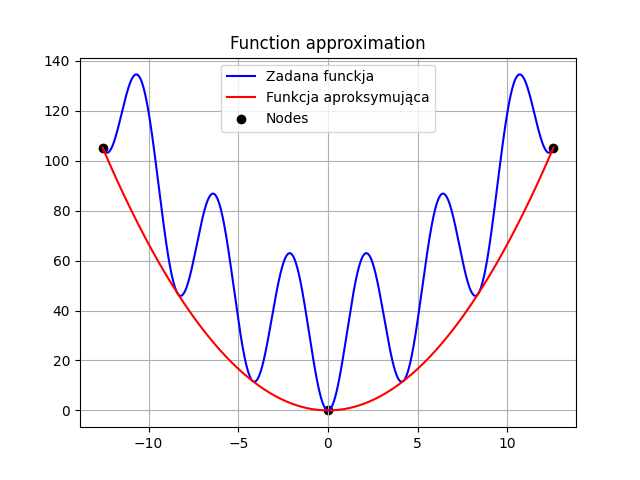
\includegraphics[width=\textwidth]{img01.png}
    \caption{Dana funkcja}
  \end{minipage}
\end{figure}

\section{Dane techniczne}

\subsection{Pochodna funkcji dla której przeprowadzone zostało doświadczenie }

Pochodna funkcji (wykres 2)

\begin{figure}[H]
  \centering
  \begin{minipage}[b]{0.3\textwidth}
    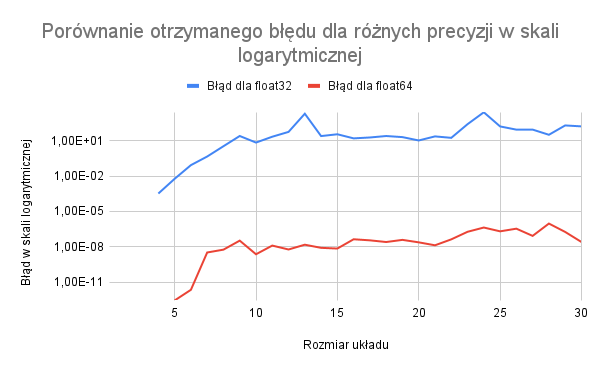
\includegraphics[width=\textwidth]{img02.png}
    \caption{Dana funkcja}
  \end{minipage}
\end{figure}

\subsection{Hardware}

Laptop z systemem operacyjnym Linux Mint, procesorem AMD Ryzen 5 5500U 2.1 GHZ oraz 8 GB pamięci RAM.

\subsection{Software}

Wykorzystany został system Pop!\_OS x64 oraz język Python w wersji 3.11.8 wraz z bibliotekami:
\begin{itemize}
\item math
\item copy
\item matplotlib
\item numpy
\end{itemize}

\section{Metody interpolacji}

\subsection{Interpolacja Lagrange'a}

Wielomian interpolacyjny Lagrange'a można wyrazić wzorem:
\[\sum_{k=0}^{n} f(\mathrm{x}_{k}^{})\mathrm{L}_{k}^{}\]
gdzie:
\bigbreak
\( f(\mathrm{x}_{k}^{})\ -\ wartości\ funkcji\ w\ punktach\ \mathrm{x}_{k}^{} \)
\bigbreak
\( \mathrm{L}_{k}^{}(x) = \frac{d}{m} = \prod_{i\ =\ 0, i\ !=\ k}^{n}\ \frac{x -\mathrm{x}_{i}^{}}{\mathrm{x}_{k}^{} - \mathrm{x}_{i}^{}}\ - \ baza\ Lagrange'a\)

\subsection{Interpolacja Newtona}

WIelomian interpolacyjny Newtowna można wyrazić wzorem:

\[ \mathrm{P}_{n}^{}(x) = f[\mathrm{x}_{0}^{}] + \sum_{i = 1}^{n}f[\mathrm{x}_{0}^{}, \mathrm{x}_{1}^{}, ..., \mathrm{x}_{i}^{}]*(x - \mathrm{x}_{0}^{})*(x - \mathrm{x}_{1}^{})*...*(\mathrm{x}_{i - 1}^{})\]

\noindent
gdzie:
\bigbreak

\( f[\mathrm{x}_{i}^{}] = f(\mathrm{x}_{i}^{}) \) \newline \indent
\( f[\mathrm{x}_{i}^{}, \mathrm{x}_{i+1}^{}] = \frac{f[\mathrm{x}_{i+1}^{}]-f[\mathrm{x}_{i}^{}]}{\mathrm{x}_{i+1}^{}-\mathrm{x}_{i}^{}} \) \newline \indent
\( . \) \newline \indent
\( . \) \newline \indent
\( . \) \newline \indent
\( f[\mathrm{x}_{i}^{}, \mathrm{x}_{i+1}^{}, ..., \mathrm{x}_{i + k}^{}] =
\frac{f[\mathrm{x}_{i+1}^{}, \mathrm{x}_{i+2}^{}, ..., \mathrm{x}_{i + k}^{}] - f[\mathrm{x}_{i}^{}, \mathrm{x}_{i+1}^{}, ..., \mathrm{x}_{i + k -1}^{}]}{\mathrm{x}_{i+k}^{} - \mathrm{x}_{i}^{}} \) \newline

\subsection{Iterpolacja Hermite'a}

Wielomian interpolacyjny Hermite'a można wyrazić wzorem

\[\mathrm{H}_{n}^{}(x) = \sum_{i = 0}^{n}\mathrm{b}_{l}^{}\mathrm{p}_{l}^{}(x) = 
\sum_{i = 0}^{k}\sum_{j=0}^{\mathrm{m}_{i}^{} - 1}\mathrm{b}_{(s(i) + j)}^{} \cdot 
\mathrm{p}_{s(i) + j}^{}(x) \]

\noindent
gdzie:

\bigbreak

\(\mathrm{p}_{s(0)}^{}(x) = 1\) 

\indent

\(\mathrm{p}_{s(i) + j}^{}(x) = \mathrm{(\mathrm{x - \mathrm{x}_{0}^{}}_{}^{})}_{}^{\mathrm{m}_{0}^{}}
\mathrm{(\mathrm{x - \mathrm{x}_{1}^{}}_{}^{})}_{}^{\mathrm{m}_{1}^{}}...
\mathrm{(\mathrm{x - \mathrm{x}_{i - 1}^{}}_{}^{})}_{}^{\mathrm{m}_{i-1}^{}}
\mathrm{(\mathrm{x - \mathrm{x}_{i}^{}}_{}^{})}_{}^{\mathrm{j}_{}^{}}\)

\indent

\(
s(i) = 
\begin{cases}
    0 & \text{dla } i = 0 \\
    \mathrm{m}_{0}^{} + \mathrm{m}_{1}^{} + ... + \mathrm{m}_{i - 1}^{} & \text{dla } i > 0
\end{cases}
\)

\indent

\(i = 0, 1, ..., k\)

\indent

\(j = 0,1,...,\mathrm{m}_{i}^{} - 1\)

\indent

Współczynniki \(\mathrm{b}_{l}^{}\) to kolejne ilorazy różnicowe.

\section{Metody szacowania błędu przybliżenia funkcji}

\subsection{Największa różnica wartości funkcji}

Największa różnica między wartością funkcji interpolowanej, a funkcji interpolującej:

\begin{center}
    \(\max_{x\in [a, b]} |F(x) - \mathrm{P}_{n}^{}(x)|\)
\end{center}

\subsection{Błąd średniokwadratowy}

Suma kwadratów różnic mięcy wartością funkcji interpolowanej, a funkcji interpolującej podzielona przez liczba punktów, w których wykonujemy porównanie:

\begin{center}
\(\frac{1}{N} * \sum_{i = 1}^{N}\mathrm{(F(\mathrm{x}_{i}^{}) - \mathrm{P}_{n}^{}(\mathrm{x}_{i}^{}))}_{}^{2}\)
\end{center}

\section{Wyniki}

Błędy zostały policzone z wykorzystaniem 1000 równoodlegle wygenerowanych punktów.

\subsection{Błąd maksymalny dla węzłów z zakresu [3, 30]}

Jak widać na wykresie 3, dotyczącym węzłów równoodległych, zdecydowanie najmniejszy błąd otrzymałem dla interpolacji Hermite'a. Jego peak przypadł na ok 9/10 węzeł. Inaczej było w przypadku skorzystania z węzłów Czebyszewa (wykres 4), ponieważ wtedy największą rozbieżnośc osiągnęła własnie interpolacja Hermite'a (do 9 węzła). Jednak szybko trend się odwrócił i od ok. 10 węzła błąd był już dużo mniejszy od interpolacji Lagrange'a / Newtona.

\begin{figure}[H]
  \begin{minipage}[b]{0.49\textwidth}
    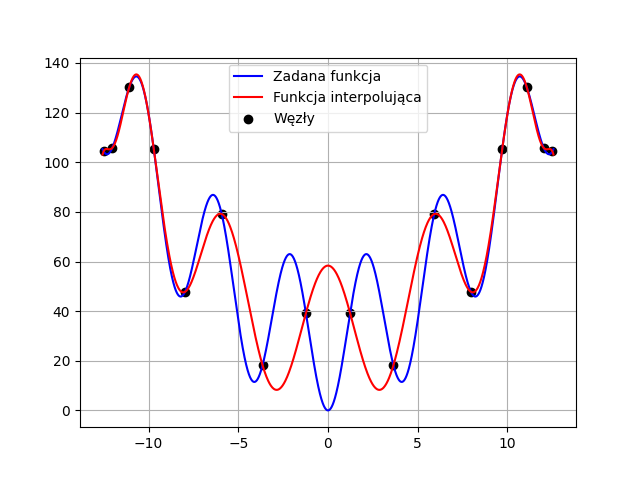
\includegraphics[width=\textwidth]{img03.png}
    \caption{Błąd maksymalny dla równoodległych węzłów}
  \end{minipage}
  \hfill
  \begin{minipage}[b]{0.49\textwidth}
    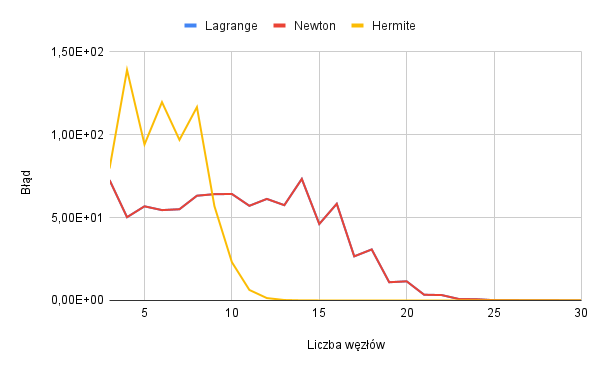
\includegraphics[width=\textwidth]{img04.png}
    \caption{Błąd maksymalny dla węzłów Czebyszewa}
  \end{minipage}
\end{figure}

Jak można zaobserwować, na powyższych wykresach nie ma niebieskiej lini, która miała oznaczać interpolację lagrange'a. Dzieje się tak, ponieważ wartości uzyskiwane przez interpolację Lagrange'a i Newtona są bardzo zbliżone, a co za tym idzie ich błędy maksymalne również. Poniżej na wykresie 5. zaprezentowana jest różnica między błędami tych dwóch interpolacji.

\begin{figure}[H]
  \centering
  \begin{minipage}[b]{0.93\textwidth}
    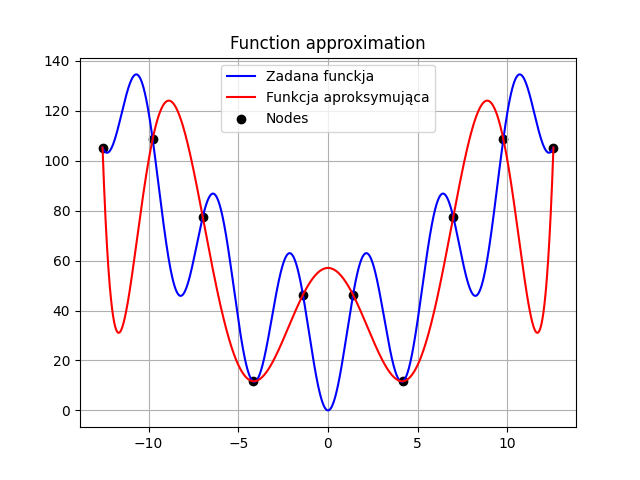
\includegraphics[width=\textwidth]{img05.png}
    \caption{Różnica między błędami interpolacji Newtona i Lagrange'a}
  \end{minipage}
\end{figure}

\subsection{Błąd maksymalny dla węzłów z zakresu [31, 70]}

Poniższe wykresy (wykres 6 i 7) prezentują błąd maksymalny dla węzłów z zakresu od 31 do 70. Zostały one wykonane w skali logarytmicznej, ze względu na ogromną rozbieżność między wartościami błędów. Jak widać interpolacja Hermite'a dla węzłów równoodległych popełnia w tym zakresie ogromny błąd w porównaniu do interpolacji Newtona i Lagrange'a. Podobniej jest dla węzłów Czebyszewa, gdzie interpolacja Hermite'a popełnia bardzo duży błąd w porównaniu do dwóch pozostałych interpolacji.

\begin{figure}[H]
  \begin{minipage}[b]{0.49\textwidth}
    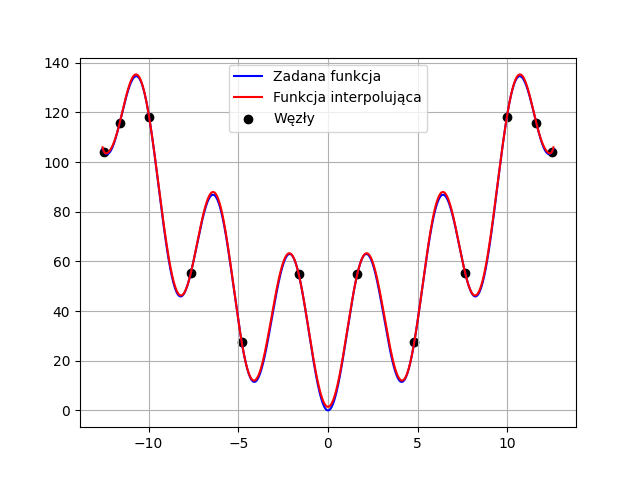
\includegraphics[width=\textwidth]{img06.png}
    \caption{Błąd maksymalny dla równoodległych węzłów}
  \end{minipage}
  \hfill
  \begin{minipage}[b]{0.49\textwidth}
    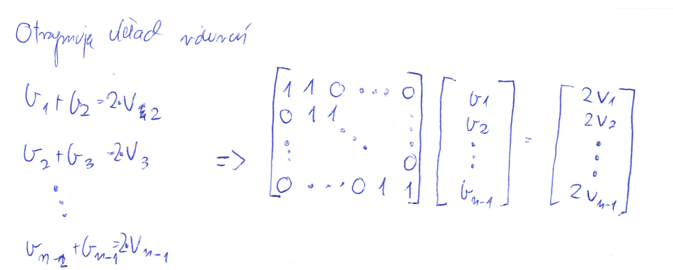
\includegraphics[width=\textwidth]{img07.png}
    \caption{Błąd maksymalny dla węzłów Czebyszewa}
  \end{minipage}
\end{figure}

Podobnie jak w zakresie 3-30, błędy interpolacji Lagrange'a i Newtona są bardzo zbliżone, co zostało pokazane poniżej na wykresie 8.

\begin{figure}[H]
  \centering
  \begin{minipage}[b]{0.93\textwidth}
    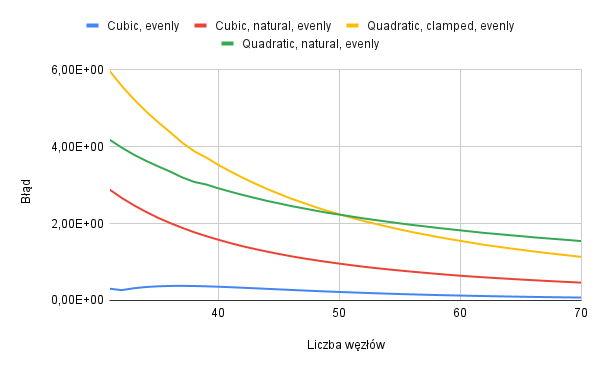
\includegraphics[width=\textwidth]{img08.png}
    \caption{Różnica między błędami interpolacji Newtona i Lagrange'a}
  \end{minipage}
\end{figure}

\subsection{Błąd średniokwadratowy dla węzłów z zakresu [3, 30]}

Peak błędu średniokwadratowego dla równoodległych węzłów przypadada na ok. 10 węzeł dla interpolacji Hermite'a, a dla interpolacji Lagrange'a / Newtona na ok. 17 węzeł (Jak widać na wykresie 9). Warto zauważyć, że dla interpolacji Hermite'a efekt Rungego jest dużo mniej widoczny. Natomiast dla węzłów Czebyszewa (wykres 10) podobnie jak w przypadku błędu maksynego, błąd średniokwadratowy dla interpolacji Hermite'a choć duży na początku szybko maleje i jest dużo mniejszy od innych interpolacji. 

\begin{figure}[H]
  \begin{minipage}[b]{0.49\textwidth}
    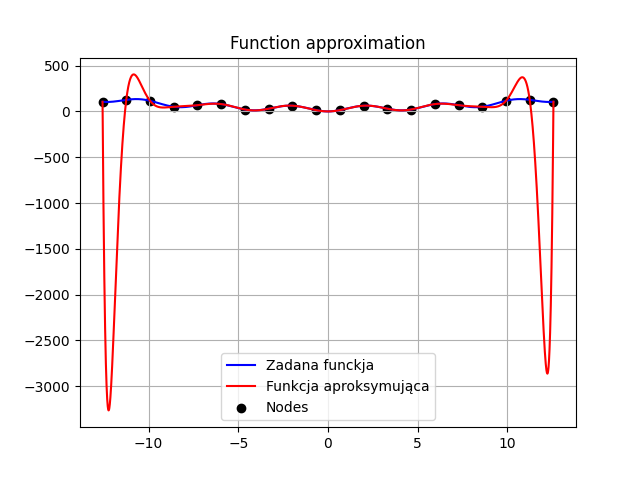
\includegraphics[width=\textwidth]{img09.png}
    \caption{Błąd średniokwadratowy dla równoodległych węzłów}
  \end{minipage}
  \hfill
  \begin{minipage}[b]{0.49\textwidth}
    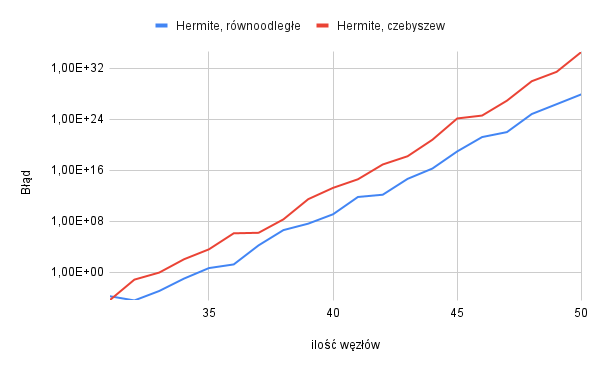
\includegraphics[width=\textwidth]{img10.png}
    \caption{Błąd średniokwadratowy dla węzłów Czebyszewa}
  \end{minipage}
\end{figure}

Jak w powyższych podpunktach błądy dla interpolacji Newtona oraz Lagrange'a są bardzo zbliżone na co dowodem jest poniższy wykres 11.

\begin{figure}[H]
  \centering
  \begin{minipage}[b]{0.93\textwidth}
    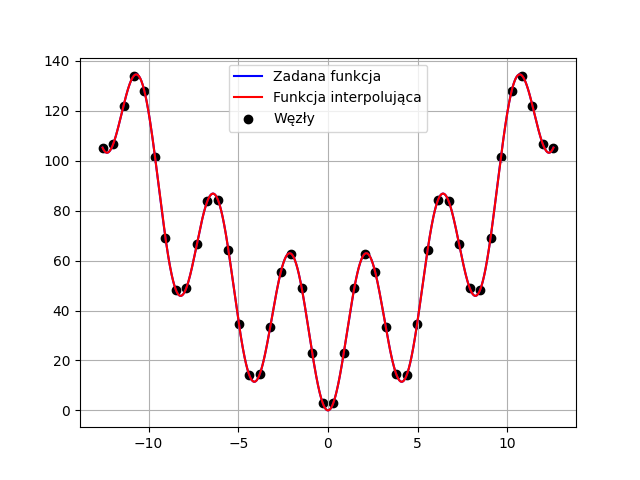
\includegraphics[width=\textwidth]{img11.png}
    \caption{Różnica między błędami interpolacji Newtona i Lagrange'a}
  \end{minipage}
\end{figure}

\subsection{Błąd średniokwadratowy dla węzłów z zakresu [31, 70]}

Jak widać na wykresie 12 dla węzłów równoodległych interpolacja Hermite'a staje się bardzo niedokładna. Zdecydowanie ciekawszy obraz kształtuje się na wykresie 13 dla węzłów Czebyszewa. Na podstawie tego wykresu można sklasyfikować dokładność trzech omawianych interpolacji w przedziale węzłów 31-70 Czwbyszewa, w kolejności od najmniej dokładnej:

\begin{itemize}
\item interpolacja Hermite'a
\item interpolacja Newtona
\item interpolacja Lagrange'a
\end{itemize}

Przy czym interpolacja Lagrange'a jest w tym przedziale bardzo dokładna, a błąd jest minimalny. 

\begin{figure}[H]
  \begin{minipage}[b]{0.49\textwidth}
    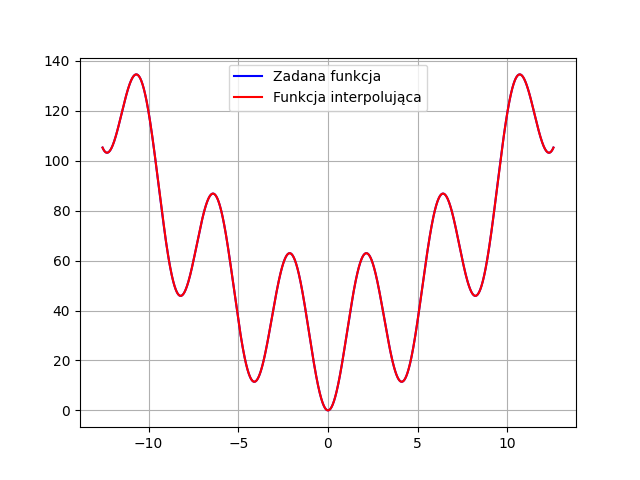
\includegraphics[width=\textwidth]{img12.png}
    \caption{Błąd średniokwadratowy dla równoodległych węzłów}
  \end{minipage}
  \hfill
  \begin{minipage}[b]{0.49\textwidth}
    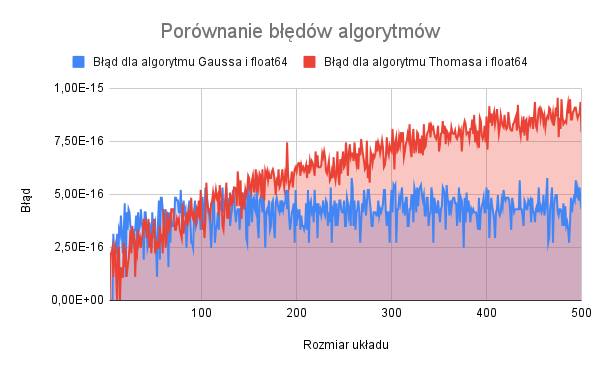
\includegraphics[width=\textwidth]{img13.png}
    \caption{Błąd średniokwadratowy dla węzłów Czebyszewa}
  \end{minipage}
\end{figure}

\subsection{Efekt Rungego}

Efekt Rungego (od nazwiska Carla Rungego, niemieckiego matematyka) – pogorszenie jakości interpolacji wielomianowej, mimo zwiększenia liczby jej węzłów. Efekt Rungego występuje tylko dla węzłów równoodległych i takie przypadki będą rozważone w tej sekcji.

\subsubsection{Interpolacja Lagrange'a i Newtona}

Jak widać na poniższym wykresie (14), efekt Rungego dla interpolacji Lagrange'a jest największy dla 17 równoodległych węzłów. Dokładnie tak samo jest w przypadku interpolacji Newtona, a wykres jest niemal identyczny (różnica niewidoczna na takim wykresie) jak w przypadku Lagrange'a.

\begin{figure}[H]
  \centering
  \begin{minipage}[b]{0.93\textwidth}
    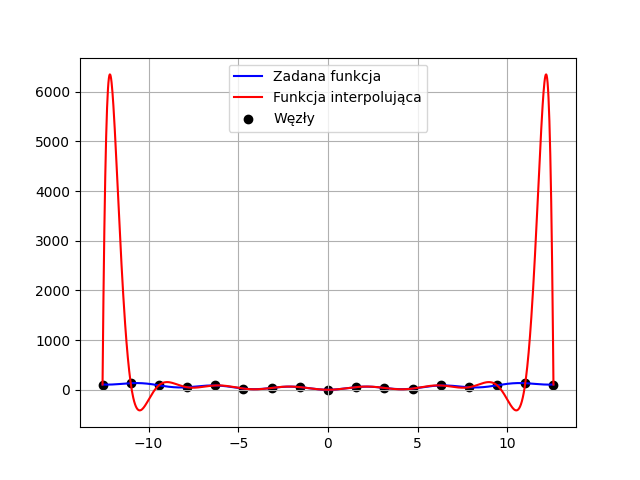
\includegraphics[width=\textwidth]{img14.png}
    \caption{Maksymalny efekt Rungego dla interpolacji Lagrange'a}
  \end{minipage}
\end{figure}

\subsubsection{Interpolacja Hermite'a}

Dla tej interpolacji efekt Rungego pojawia się wcześniej i jest dużo mniejszy, niż w przypadku dwóch pozostałych interpolacji. A więc jak widać na wykresie 15, "peak" przypada na 10 węzeł.

\begin{figure}[H]
  \centering
  \begin{minipage}[b]{0.93\textwidth}
    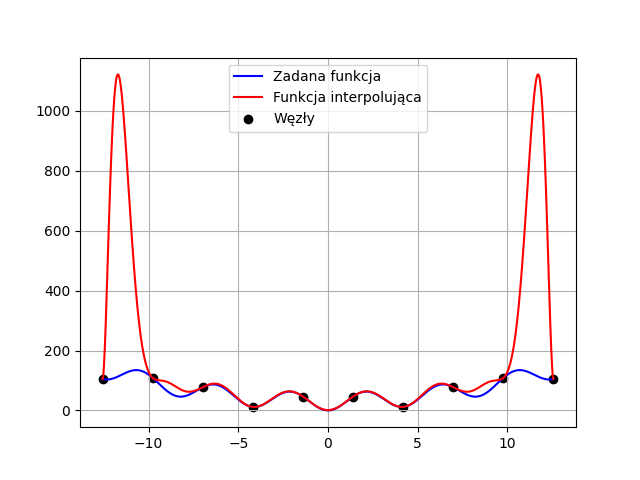
\includegraphics[width=\textwidth]{img15.png}
    \caption{Maksymalny efekt Rungego dla interpolacji Hermite'a}
  \end{minipage}
\end{figure}

\subsection{Najlepsze przybliżenie interpolowanej funkcji}

W celu łatwiejszej oceny, które przybliżenie było lepsze sporządziłem tabelkę (tabela 1), która pokazuje przy którym węźle interpolacja była na najlepszym poziomie lub od kiedy zaczynała być akceptowalna (za próg akceptowalności przyjąłem wartość błędu maksymalnego na poziomie 10E-4).

\begin{table}[!ht]

\begin{figure}[H]
  \centering
  \begin{minipage}[b]{0.93\textwidth}
    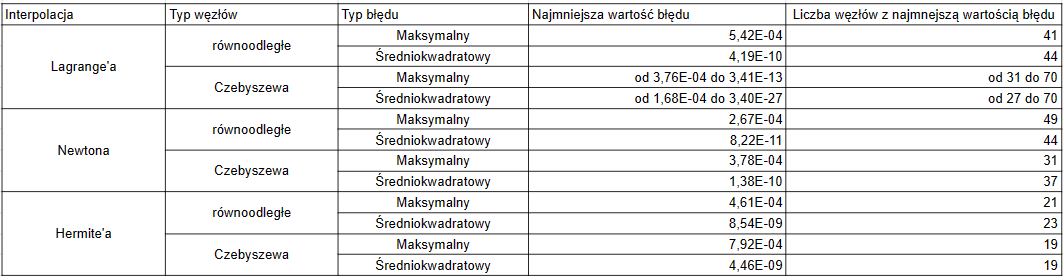
\includegraphics[width=\textwidth]{img16.png}
  \end{minipage}
\end{figure}
\caption{Najlepsze przyblizenie dla różnych interpolacji}
\end{table}

Analizując powyższą tabelkę można dojść do wniosku, że jeśli chcemy minimalizować liczbę użytych węzłów (a zazwyczaj checemy) to należy skorzystać z interpolacji Hermite'a, która dla 19 daje bardzo dobre przybliżenie. Jednak jeśli zależy nam na jak największej możliwej precyzji to trzeba skorzystać z interpolacji Lagrange'a i zwiększać liczbę węzłów, aż osiągniemy zamieżoną precyzję.

Przybliżenie otrzymane dla 19 węzłów Czebyszewa i interpolacji Hermite'a to zostało zaprezentowane na ponizszym wykresie (17).

\begin{figure}[H]
  \centering
  \begin{minipage}[b]{0.93\textwidth}
    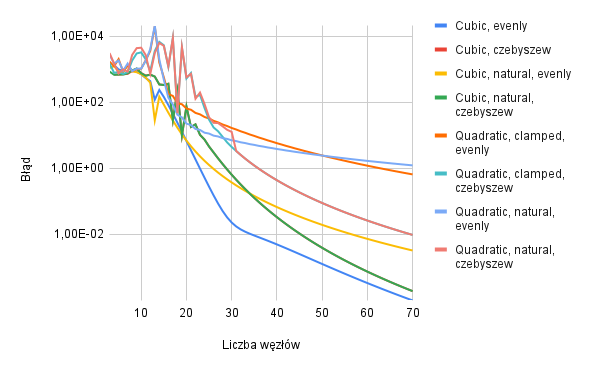
\includegraphics[width=\textwidth]{img17.png}
    \caption{Najlepsze przyblizenie interpolowanej funkcji}
  \end{minipage}
\end{figure}

\subsection{Wybrane wartości błędów interpolacji}

Poniżej w tabelach 2, 3, 4, 5, 6, 7 pokazane są wybrane wartości błędów interpolacji w celu jeszcze lepszego zobrazowania z jakimi rzędami wartości mamy do czynienia

\subsubsection{Interpolacja Lagrange'a - Błąd maksymalny}

Jak można zauważyć, węzły Czebyszewa są zdecydowanie lepszym rozwiązaniem dla interpolacji Lagrange'a

\begin{table}[H]
    \centering
    \begin{tabular}{|r|r|r|}
    \hline
        Liczba węzłów / Metoda interpolacji & Lagrange, w. równoodległe & lagrange, w. Czebyszewa  \\ \hline
        10 & 8,71E+01 & 6,43E+01  \\ \hline
        20 & 2,88E+03 & 1,15E+01  \\ \hline
        30 & 2,28E+01 & 2,34E-03  \\ \hline
        40 & 3,01E-03 & 8,31E-09  \\ \hline
        50 & 1,23E-02 & 1,99E-13  \\ \hline
        60 & 9,19E+00 & 2,84E-13  \\ \hline
        70 & 8,49E+03 & 3,41E-13 \\ \hline
    \end{tabular}
    \caption{Wybrane wartości błędu maksymalnego dla interpolacji Lagrange'a}
\end{table}

\subsubsection{Interpolacja Lagrange'a Błąd średniokwadratowy}

Na przykładzie błędu średniokwadratowego wyższość węzłów Czebyszewa jest jeście bardziej widoczna (tabela 3).

\begin{table}[H]
    \centering
    \begin{tabular}{|r|r|r|}
    \hline
        Liczba węzłów / Metoda interpolacji & lagrange, w. równoodległe & lagrange, w. Czebyszewa  \\ \hline
        10 & 1,89E+03 & 8,29E+02  \\ \hline
        20 & 3,52E+05 & 3,25E+01  \\ \hline
        30 & 1,34E+01 & 2,07E-06  \\ \hline
        40 & 1,65E-07 & 2,98E-17  \\ \hline
        50 & 5,74E-07 & 2,49E-27  \\ \hline
        60 & 4,22E-01 & 4,22E-27  \\ \hline
        70 & 3,34E+05 & 3,40E-27 \\ \hline
    \end{tabular}
    \caption{Wybrane wartości błędu średniokwadratowego dla interpolacji Lagrange'a}
\end{table}

\subsubsection{Interpolacja Newtona'a - Błąd maksymalny}

Jak widać po poniższej tabeli (4), wartości błędów dla interpolacji Newtona są dość zbliżone.

\begin{table}[H]
    \centering
    \begin{tabular}{|r|r|r|}
    \hline
        Liczba węzłów / Metoda interpolacji  & Newton, w. równoodległe & Newton, w. Czebyszewa  \\ \hline
        10  & 8,71E+01 & 6,43E+01  \\ \hline
        20  & 2,88E+03 & 1,15E+01  \\ \hline
        30  & 2,28E+01 & 2,34E-03  \\ \hline
        40  & 3,03E-03 & 1,68E-04  \\ \hline
        50  & 5,09E-04 & 2,32E-03  \\ \hline
        60  & 1,23E-01 & 3,23E-02  \\ \hline
        70 & 4,57E+02 & 8,77E+02 \\ \hline
    \end{tabular}
    \caption{Wybrane wartości błędu maksymalnego dla interpolacji Newtona'a}
\end{table}

\subsubsection{Interpolacja Newton'a - Błąd średniokwadratowy}

Podobnie, jak w przypadku błędu maksymalnego wartości są dość zbliżone (tabela 5).

\begin{table}[H]
    \centering
    \begin{tabular}{|r|r|r|}
    \hline
        Liczba węzłów / Metoda interpolacji & Newton, w. równoodległe & Newton, w. Czebyszewa  \\ \hline
        10 & 1,89E+03 & 8,29E+02  \\ \hline
        20 & 3,52E+05 & 3,25E+01  \\ \hline
        30 & 1,34E+01 & 2,07E-06  \\ \hline
        40 & 1,68E-07 & 3,86E-10  \\ \hline
        50 & 3,45E-09 & 4,39E-08  \\ \hline
        60 & 8,70E-05 & 9,62E-06  \\ \hline
        70 & 1,40E+03 & 5,50E+03 \\ \hline
    \end{tabular}
    \caption{Wybrane wartości błędu średniokwadratowego dla interpolacji Newtona'a}
\end{table}

\subsection{Interpolacja Hermite'a - Błąd maksymalny}

Jak widać w tabeli 6, wartości rosną do ogromnych rzędów i interpolacja Hermite'a staje się bezużyteczna już od 30 / 40 węzłów.

\begin{table}[H]
    \centering
    \begin{tabular}{|r|r|r|}
    \hline
        Liczba węzłów / Metoda interpolacji  & Hermite, w. równoodległe & Hermite, w. Czebyszewa  \\ \hline
        10  & 1,01E+03 & 2,31E+01  \\ \hline
        20  & 1,03E-03 & 1,56E-03  \\ \hline
        30  & 3,33E-02 & 4,60E-02  \\ \hline
        40  & 7,16E+05 & 5,22E+07  \\ \hline
        50  & 2,09E+15 & 3,47E+18  \\ \hline
        60  & 1,15E+25 & 2,85E+28  \\ \hline
        70 & 9,59E+33 & 3,37E+38 \\ \hline
    \end{tabular}
    \caption{Wybrane wartości błędu maksymalnego dla interpolacji Hermite'a}
\end{table}

\subsection{Interpolacja Hermite'a - Błąd średniokwadratowy}

Podobnie jak dla błędu maksymalnego widać ogromne wartości błędów (tabela 7).

\begin{table}[!ht]
    \centering
    \begin{tabular}{|r|r|r|}
    \hline
        Liczba węzłów / Metoda interpolacji & Hermite, w. równoodległe & Hermite, w. Czebyszewa  \\ \hline
        10 & 7,43E+04 & 9,75E+01  \\ \hline
        20 & 1,75E-08 & 1,29E-08  \\ \hline
        30 & 1,87E-05 & 1,56E-05  \\ \hline
        40 & 1,20E+09 & 1,70E+13  \\ \hline
        50 & 8,65E+27 & 4,01E+34  \\ \hline
        60 & 2,95E+47 & 2,20E+54  \\ \hline
        70 & 1,89E+65 & 3,00E+74 \\ \hline
    \end{tabular}
\end{table}

\section{Wnioski}

\begin{itemize}
\item W celu uzyskania dobrego przyblizenia przy dość małej liczbie węzłów należy skorzystać z interpolacji Hermite'a z węzłami Czebyszewa
\item W celu uzyskania bardzo dokładnego przybliżenia należy skorzystać z interpolacji Lagrange'a z węzłani Czebyszewa, jednak trzeba liczyć się z tym, że liczba węzłów będzie dość duża
\item Interpolacje na równoodległych węzłach są obarczone dużym błędem ze względu na efekt Rungego
\item Algorytm Newtona oraz Hermite'a przy dużej ilości węzłów zaczyna generować ogromne błędy z uwagi na niedokładną reprezentacje liczb zmiennoprzecinkowych
\item Węzły Czebyszewa dają lepsze wyniki od węzłów równoodległych
\item Błąd maksymalny pozwala trafnie określić, gdzie zachodzi efekt Rungego (dla małej ilości węzłów). Dla dużej ilości węzłów bardzo widoczny jest problem z reprezentacją liczb zmiennoprzecinkowych w komputerze, ponieważ otrzmane wartości błędów są ogromne
\item Każdy algorytm interpolacji ma swoje wady i zalety, dlatego też każdy może być użyteczy w zależnośći od efektu jaki chcemy osiągnąć (np. minimalizacja liczby węzłów, minimalizacja błędu przybliżenia), zatem nie ma jednego nalepszego algorytmu.
\end{itemize}


\end{document}
